VueJS ist ein JavaScript Framework, welches verwendet wird um Benutzeroberflächen zu bauen. Dafür baut es auf nativen HTML, CSS und JavaScript und ermöglicht dabei ein deklaratives und Komponenten basiertes Programmiermodel. 
\cite{frontend_web_vuejs_introduction}

\subsubsection{Model View ViewModel}
VueJS verwendet das MVVM-Prinzip, welches es gibt um zwischen der grundlegenden Benutzeroberfläche eines Projektes, der direkten Oberflächenlogik für die Veranschaulichung von Informationen und der tieferen Logik zu unterscheiden. Diese klare strukturierte Trennung sorgt auch dafür, dass VueJS mit einem sogenannten Build-Tool so gebaut werden kann, dass nicht verwendete Teile des Codes nicht ausgeliefert werden und somit die Geschwindigkeit maximiert wird. 

\begin{figure}[h]
    \centering
    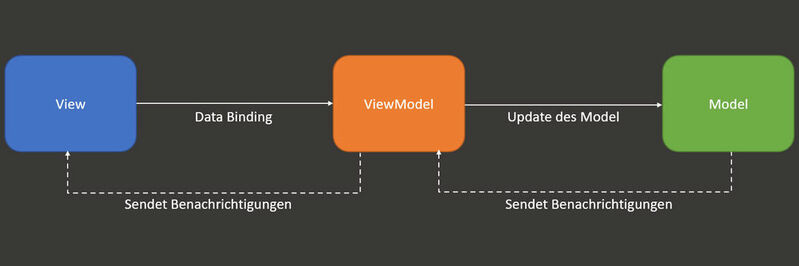
\includegraphics[width=1\textwidth]{pics/vuejs-mvvm.jpeg}
    \caption{MVVM Ablauf}
    \cite{frontend_web_mvvm}
    \label{fig:mesh1}
\end{figure}

\cite{frontend_web_mvvm}

\subsubsection{Komponenten}
Ein sehr fundamentaler Punkt des Frameworks sind die Komponenten. In VueJS werden verschiedene Abschnitte in einzelne Komponenten ausgelagert. Dies sorgt für eine einheitliche Struktur und bietet den Programmierern eine bessere Übersicht, da jede Datei eindeutig erkennbar ist und durch die Abtrennung in der Regel nicht zu groß ist. Jede Komponente endet dabei mit \textbf{.vue} und hat den selben Grundaufbau:

\newpage
\cite{frontend_web_vuejs_components}
\newline

\begin{lstlisting}[language=html]
    <template>
    <!-- HTML Code -->
    </template>
    
    <script>
    // JavaScript Code
    </script>
    
    <style scoped>
    /* CSS Code */
    </style>
\end{lstlisting}

Wie in dem Code-Beispiel zu sehen ist, werden in jeder Komponente HTML, Javascript und CSS klar abgetrennt. Bei dem \textbf{style} Tag gibt es hierbei noch die optionale Option \textbf{scoped}, die dafür sorgt, das die CSS-Regeln nur in dieser Komponente angewendet werden. Wenn dies nicht so ist, wird dies im ganzen Projekt global verwendet, das kann jedoch zu Komplikationen führen, da im Nachhinein nicht mehr nachvollziehbar ist, wo welche CSS-Regeln definiert wurde.

\cite{frontend_web_vuejs_components2}

\subsubsection{Options-API vs Compositon-API}
In VueJS gibt es zwei verschiedene Arten zu programmieren. Dabei gibt es die Options-API und die Composition API, welche sich hauptsächlich in der Syntax unterscheiden. Die Composition-API ist eine neue Funktion, die es seit VueJS 3 gibt und gibt dem Programmierer:in eine neue Möglichkeit Logik in Komponenten zu definieren. Dadurch ist es möglich einen funktionalen Programmierstyle zu verwenden und Logik über mehrere Komponenten zu verwenden. Die Options-API hingegen ist der traditionelle Weg um die Logik von Komponenten zu definieren. Hierbei ist der Programmierstyle sehr objektorientiert. Grundlegend bietet die Composition-API viel mehr Freiheiten, da nicht mehr festgelegt wird, wo welche Logik genau implementiert werden muss.
\newpage
\begin{lstlisting}
    import { ref, computed } from 'vue'

    export default {
      setup() {
        const count = ref(0)
    
        const increment = () => {
          count.value++
        }
    
        const double = computed(() => {
          return count.value * 2
        })
    
        return {
          count,
          increment,
          double
        }
      }
    }
\end{lstlisting}
\newline
\begin{lstlisting}
    export default {
      data() {
        return {
          count: 0
        }
      },
      methods: {
        increment() {
          this.count++
        }
      },
      computed: {
        double() {
          return this.count * 2
        }
      }
    }
\end{lstlisting}
Beim ersten Code-Beispiel handelt es sich um die Compositon-API und im zweiten um die Options-API. Wie man sehen kann muss bei Verwendung der Options-API alles in vordefinierte Blöcke bestimmt werden, bei der Composition-API ist dies nicht der Fall.

\cite{frontend_web_vuejs_api}

\subsubsection{Reactivity System}
VueJS verwendet ein sogenanntes Reactivity-System, welches zu einem der wichtigsten Feature des Frameworkes zählt. Dieses System sorgt dafür, dass sich JavaScript Variablen wenn sie geändert werden live in der Benutzeroberfläche updaten und das ohne Page-Reload. Die Basis bieten hierbei JavaScript Proxys, wobei ein Handler mit Getter- und Settermethoden verwendet wird. 
\newpage
\begin{lstlisting}[language=html]
    <script>
    export default {
      data() {
        return {
          count: 0
        }
      },
      methods: {
        increment() {
          this.count++
        }
      }
    }
    </script>
    
    <template>
      <button @click="increment">Zaehler: {{ count }}</button>
    </template>
\end{lstlisting}

\cite{frontend_web_vuejs_reactivity}

In diesem Beispiel sieht man im ersten Abschnitt wie eine Variable mit dem Namen “count” erstellt wird und den Wert 0 zugewiesen bekommt. Dies passiert in der data-Funktion, welche alle Variablen reactive macht. Ebenfalls wurde eine Methode names “increment” erstellt, welche auf die count-Variable zugreift und diese beim Aufruf einmal erhöht. Im HTML wurde ein \textbf{<button>} Tag erstellt, welcher einen Text beinhaltet und die count-Variable gebindet hat. Ebenfalls liegt auf dem Element ein Eventlistener, welcher einen Klick abfängt und dann die increment Methode aufruft.
Aufgrund der Reaktivität wird die count Variable nun beim Klicken des Buttons jeweils erhöht und zeitgleich im HTML richtig angezeigt. Diese Logik passiert ohne Page-Reload.

\cite{frontend_web_vuejs_reactivity2}

\subsubsection{Lifecycle-Hooks}
VueJS bietet mit Lifecycle-Hooks ebenfalls sehr essentielle Funktionalitäten. Damit kann bestimmt werden, wann eine Komponente erstellt, im DOM hinzugefügt, zerstört oder auch aktualisiert wird. 
\newpage
\begin{figure}[h!]
    \centering
    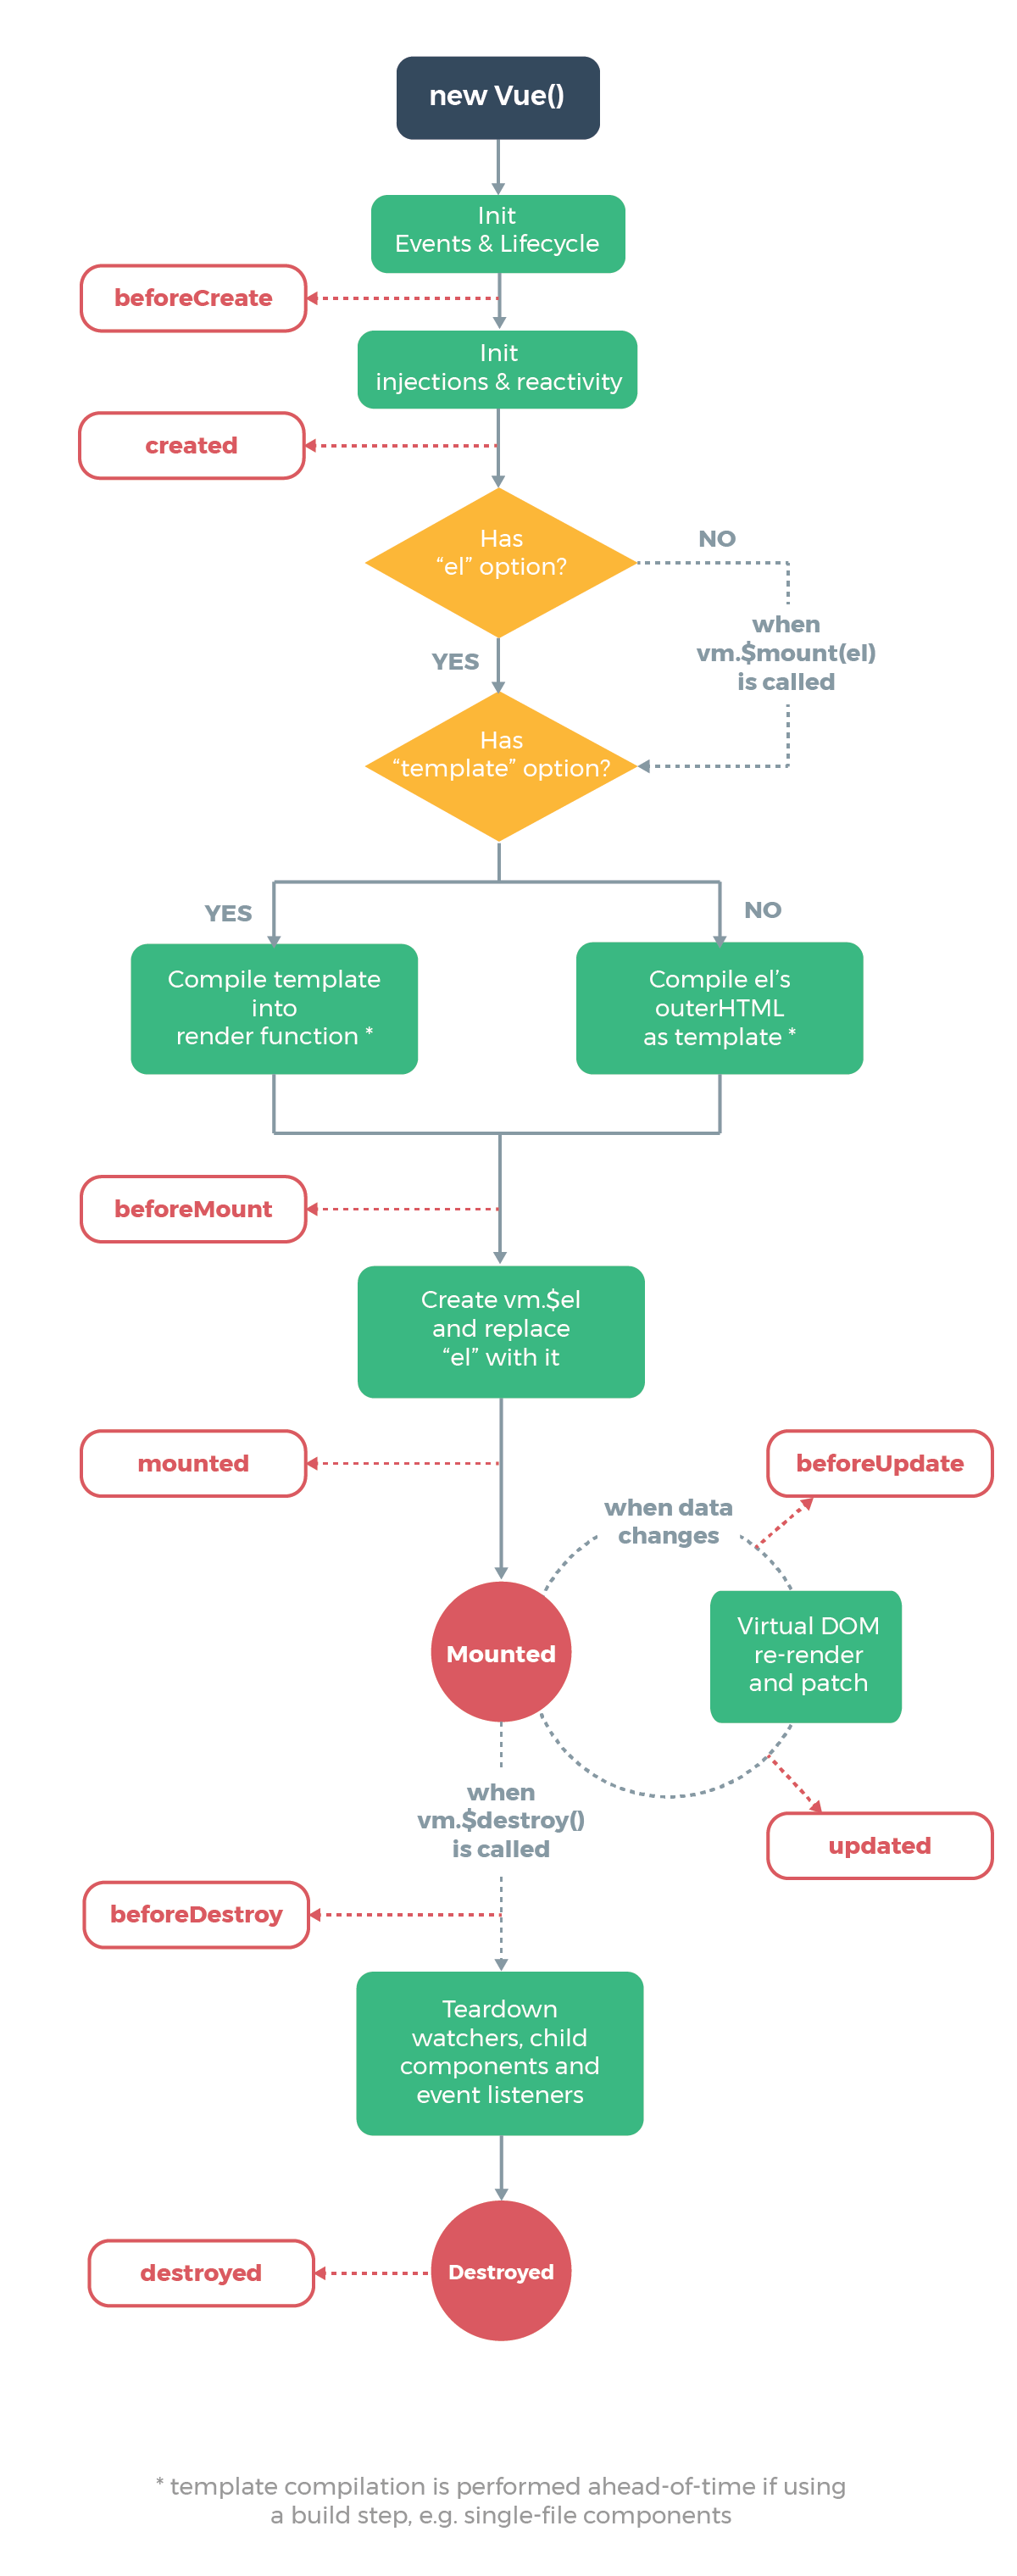
\includegraphics[width=0.6\textwidth]{pics/vuejs-lifecycle.png}
    \caption{VueJS Lifecycle}
    \cite{frontend_web_vuejs_lifecycle}
    \label{fig:mesh1}
\end{figure}

In dieser Grafik ist ein sogenannter Instance-Lifecycle zu sehen, worin alle Lifecycle-Hooks zu finden sind.

\subsubsection{Creation Hooks}
Hierbei handelt es sich um die erste Hook, die eine Komponente ausführt. Damit können Aktionen bestimmt werden, welche dann ausgeführt werden bevor die Komponente im DOM eingebaut wird. Dadurch hat man in dieser Hook dementsprechend auch keinen Zugriff auf das DOM.
Dies kann in VueJS mit \textbf{beforeCreate} abgefangen werden.

\begin{lstlisting}
    <script>
    export default {
    	beforeCreate() {
    		console.log('beforeCreate Hook')
    	}
    }
    </script>
\end{lstlisting}

Diese Funktion wird nun während der Initialisierung einer Komponente ausgeführt. Daten sind zu diesem Zeitpunkt noch nicht reaktiv und Ereignisse sind noch nicht initialisiert.
Zusätzlich gibt es die \textbf{created} Methode:

\begin{lstlisting}
    <script>
    export default {
      data() {
        return {
          property: 'Hello'
        }
      },
      created() {
        this.property = 'Hello world!'
      }
    }
    </script>
\end{lstlisting}

In dieser Methode sind Daten schon reaktiv und man kann darauf zugreifen. In diesem Beispiel wird die Variable \textbf{property} von ‘Hello’ auf ‘Hello world!’ geändert. Der DOM ist dabei jedoch noch nicht erreichbar.

\subsubsection{Mounting Hooks}
Die Mounting Hooks werden am meisten verwendet und ermöglichen den Zugriff auf die Komponente vor oder nach dem ersten Rendern.

In VueJS gibt es hierbei zuerst die \textbf{beforeMount} Hook, welche aufgerufen wird bevor das erste Rendern stattgefunden hat.

\begin{lstlisting}[language=html]
    <script>
    export default {
      beforeMount() {
        console.log(`Zu diesem Zeitpunkt wurde vm.$el noch nicht erstellt.`)
      }
    }
    </script>
\end{lstlisting}

In diesem Beispiel wird in der Konsole ausgegeben, dass \textbf{vm.el} noch nicht erstellt worden ist. Dies ist das Property, welches auf den DOM zugreifen kann. 

Zusätzlich gibt es die \textbf{mounted} Hook, welche nach dem ersten Rendern aufgerufen wird. Dadurch hat man das erste Mal die Möglichkeit auf die vollständige reaktive Komponente oder auch das DOM zuzugreifen.

\begin{lstlisting}
    <template>
      <div ref="example-element">Example component.</div>
    </template>
    
    <script>
    export default {
      mounted() {
        console.log(this.$el.textContent)
      }
    }
    </script>
\end{lstlisting}

In diesem Code Beispiel wird in der mounted-Methode auf das DOM zugegriffen und der Inhalt des definierten \textbf{<div>} in der Konsole ausgegeben.

\subsubsection{Updating Hooks}
Diese Hooks werden aufgerufen wenn sich eine reaktive Eigenschaft ändert und damit ein erneutes Rendering benötigt wird.

In VueJS gibt es die \textbf{beforeUpdate} Methode, welche nach der Änderung einer solchen reaktiven Eigenschaft ausgeführt wird. Zu diesem Zeitpunkt wurde das DOM noch nicht neu gerendert. Dadurch wird diese Hook verwendet, um geänderte reaktive Daten zu sehen bevor diese in das DOM geladen werden.

\begin{lstlisting}
    <template>
      <div ref="example-element">{{counter}}</div>
    </template>
    
    <script>
    export default {
      data() {
        return {
          counter: 0
        }
      },
      created() {
        setInterval(() => {
          this.counter++
        }, 1000)
      },
      beforeUpdate() {
        console.log(this.counter)
      }
    }
    </script>
\end{lstlisting}

In diesem Beispiel wird die Variable \textbf{counter} 1000ms nach Erstellung der Komponente erhöht. Dadurch wird \textbf{beforeUpdate} aufgerufen, in welcher die neue Variable in der Konsole ausgegeben wird. Wenn diese Ausgabe geschieht hat die Variable zwar einen neuen Wert, wurde jedoch im HTML noch nicht aktualisiert.
\newpage
Um nun auch den Zeitpunkt nach dem Rendern des neuen DOM abzufangen gibt es die \textbf{updated} Hook.

\begin{lstlisting}
    <template>
      <div ref="example-element">{{counter}}</div>
    </template>
    
    <script>
    export default {
      data() {
        return {
          counter: 0
        }
      },
      created() {
        setInterval(() => {
          this.counter++
        }, 1000)
      },
      updated() {
        console.log(+this.$refs['example-element'].textContent === this.counter)
      }
    }
    </script>
\end{lstlisting}

Dieses Beispiel ist von der Funktionalität gleich wie das Vorige. Der einzige Unterschied besteht darin, dass hierbei die \textbf{updated} Methode aufgerufen wird. In dieser wird der Wert von \textbf{counter} direkt aus dem DOM genommen und mit dem Wert der tatsächlichen Variable verglichen. Das Ergebnis wird in der Konsole ausgegeben und ergibt \textbf{true}. Grund dafür ist, dass in dieser Hook, das DOM bereits neu gerendert wurde und somit schon den neuen Wert angenommen hat.

\subsubsection{Destruction Hooks}
Die sogenannten Destruction Hooks ermöglichen die Ausführung von Aktionen, wenn eine Komponente zerstört wird. Diese können wichtig sein um beispielsweise noch Daten am Ende zu speichern oder auch um bestimmte Daten zu bereinigen.
In VueJS gibt es hierfür zwei Hooks. Die erste ist die \textbf{beforeDestroy} Methode.

\begin{lstlisting}
    <script>
    export default {
      data() {
        return {
          exampleLeakyProperty: 'Hello World!'
        }
      },
    
      beforeDestroy() {
        this.exampleLeakyProperty = null
        delete this.exampleLeakyProperty
      }
    }
    </script>
\end{lstlisting}

Zu diesem Zeitpunkt ist die Komponente noch normal funktionell und es sind alle Daten noch vorhanden. In diesem Beispiel wird eine Variable manuell gelöscht, bevor die Komponente zerstört wird.
\newpage
Des weiteren gibt es noch die \textbf{destroyed} Hook.

\begin{lstlisting}
    <script>
    import ExampleAnalyticsService from './example-analytics-service'
    
    export default {
      destroyed() {
        ExampleAnalyticsService.informService('Komponente zerstört.')
      }
    }
    </script>
\end{lstlisting}

Zu diesem Zeitpunkt wurde die Komponente schon vollständig abgebaut,  die Methode kann zum Beispiel verwendet werden um einen externen Services zu informieren, dass die Komponente zerstört wurde.

\cite{frontend_web_vuejs_lifecycle}